% !TEX program = xelatex
% In emacs, use this to set default compiler to xelatex:
% M-x TeX-engine-set RET xetex RET

\documentclass[xcolor=table,aspectratio=169]{beamer}

\usepackage{fancyvrb}
\usepackage{array}
\usepackage{booktabs}

\setbeamertemplate{navigation symbols}{}

\usepackage{listings}

\usepackage{graphicx}
\usepackage{hanging}
\usepackage{natbib} %citep and citet
\usepackage{amsmath}
\usepackage{mathtools}

\usepackage{xltxtra}
\setsansfont{Arial}
\setmonofont[Mapping=tex-text]{Fira Code}

\bibliographystyle{apalike}

\usetheme{Amsterdam2}
\usecolortheme{rose}
%%%%%%%%%%%%%%%%%%%%%%%%%%%%%%%%%%%%%%%%%%%

\usepackage{fancyvrb}
\newcommand{\VerbBar}{|}
\newcommand{\VERB}{\Verb[commandchars=\\\{\}]}
\DefineVerbatimEnvironment{Highlighting}{Verbatim}{commandchars=\\\{\}}
% Add ',fontsize=\small' for more characters per line
\usepackage{framed}
\definecolor{shadecolor}{RGB}{248,248,248}
\newenvironment{Shaded}{\begin{snugshade}}{\end{snugshade}}
\newcommand{\KeywordTok}[1]{\textcolor[rgb]{0.13,0.29,0.53}{\textbf{{#1}}}}
\newcommand{\DataTypeTok}[1]{\textcolor[rgb]{0.13,0.29,0.53}{{#1}}}
\newcommand{\DecValTok}[1]{\textcolor[rgb]{0.00,0.00,0.81}{{#1}}}
\newcommand{\BaseNTok}[1]{\textcolor[rgb]{0.00,0.00,0.81}{{#1}}}
\newcommand{\FloatTok}[1]{\textcolor[rgb]{0.00,0.00,0.81}{{#1}}}
\newcommand{\ConstantTok}[1]{\textcolor[rgb]{0.00,0.00,0.00}{{#1}}}
\newcommand{\CharTok}[1]{\textcolor[rgb]{0.31,0.60,0.02}{{#1}}}
\newcommand{\SpecialCharTok}[1]{\textcolor[rgb]{0.00,0.00,0.00}{{#1}}}
\newcommand{\StringTok}[1]{\textcolor[rgb]{0.31,0.60,0.02}{{#1}}}
\newcommand{\VerbatimStringTok}[1]{\textcolor[rgb]{0.31,0.60,0.02}{{#1}}}
\newcommand{\SpecialStringTok}[1]{\textcolor[rgb]{0.31,0.60,0.02}{{#1}}}
\newcommand{\ImportTok}[1]{{#1}}
\newcommand{\CommentTok}[1]{\textcolor[rgb]{0.56,0.35,0.01}{\textit{{#1}}}}
\newcommand{\DocumentationTok}[1]{\textcolor[rgb]{0.56,0.35,0.01}{\textbf{\textit{{#1}}}}}
\newcommand{\AnnotationTok}[1]{\textcolor[rgb]{0.56,0.35,0.01}{\textbf{\textit{{#1}}}}}
\newcommand{\CommentVarTok}[1]{\textcolor[rgb]{0.56,0.35,0.01}{\textbf{\textit{{#1}}}}}
\newcommand{\OtherTok}[1]{\textcolor[rgb]{0.56,0.35,0.01}{{#1}}}
\newcommand{\FunctionTok}[1]{\textcolor[rgb]{0.00,0.00,0.00}{{#1}}}
\newcommand{\VariableTok}[1]{\textcolor[rgb]{0.00,0.00,0.00}{{#1}}}
\newcommand{\ControlFlowTok}[1]{\textcolor[rgb]{0.13,0.29,0.53}{\textbf{{#1}}}}
\newcommand{\OperatorTok}[1]{\textcolor[rgb]{0.81,0.36,0.00}{\textbf{{#1}}}}
\newcommand{\BuiltInTok}[1]{{#1}}
\newcommand{\ExtensionTok}[1]{{#1}}
\newcommand{\PreprocessorTok}[1]{\textcolor[rgb]{0.56,0.35,0.01}{\textit{{#1}}}}
\newcommand{\AttributeTok}[1]{\textcolor[rgb]{0.77,0.63,0.00}{{#1}}}
\newcommand{\RegionMarkerTok}[1]{{#1}}
\newcommand{\InformationTok}[1]{\textcolor[rgb]{0.56,0.35,0.01}{\textbf{\textit{{#1}}}}}
\newcommand{\WarningTok}[1]{\textcolor[rgb]{0.56,0.35,0.01}{\textbf{\textit{{#1}}}}}
\newcommand{\AlertTok}[1]{\textcolor[rgb]{0.94,0.16,0.16}{{#1}}}
\newcommand{\ErrorTok}[1]{\textcolor[rgb]{0.64,0.00,0.00}{\textbf{{#1}}}}
\newcommand{\NormalTok}[1]{{#1}}

%%%%%%%%%%%%%%%%%%%%%%%%%%%%%%%%%%%%%%%%%%%%%
\usepackage{color}
\definecolor{mygreen}{rgb}{0,0.6,0}
\definecolor{mygray}{rgb}{0.5,0.5,0.5}
\definecolor{mymauve}{rgb}{0.58,0,0.82}
\definecolor{ForestGreen}{rgb}{0.13,0.54,0.13}

\beamersetuncovermixins{\opaqueness<1>{25}}{\opaqueness<2->{15}}


%%186     206     17      38      #CE1126                    

\title[Supervised learning-classification (1/2)]{
	{\LARGE{Statistical learning and Visualization}:\\\large{Supervised learning - classification (1/2)}}
}
\institute{
	\footnotesize Department of Methodology and Statistics\\
}
\author[van Kesteren]{Erik-Jan van Kesteren}
\date{
\includegraphics[height=1.5cm]{pics/uu-logo.png}\\
	
	\footnotesize{\emph{Applied Data Science}}}


\newcommand{\referto}[1]{\hfill{\scriptsize{\emph{\color{gray}{#1}}}}}


\begin{document}

\begin{frame}
\maketitle
\end{frame}

\begin{frame}
  \tableofcontents
\end{frame}

\section{Introduction}\subsection{}

\begin{frame}{About me}
	\begin{itemize}
		\item Assistant professor of data science @ UU M\&S
		\item Team lead for the Social Data Science Team (ODISSEI national consortium)
		\item Statistics, programming, high-dimensional data, geospatial analysis, supercomputing, structural equation modeling, (Bayesian) probabilistic programming, optimization, synthetic data, and more
		\item I will teach two classification weeks in this course
		\item I coordinate the \texttt{INFOMDA2} course (sign up everyone)!
	\end{itemize}
\end{frame}

\begin{frame}{Topics this week}
	\begin{itemize}
		\item Classification
		\item KNN
		\item Logistic regression
		\item Linear discriminant analysis
		\item Generative vs discriminative
		\item Trees
		\item Confusion matrix
	\end{itemize}
\end{frame}

\begin{frame}
	{Classification}
	
	The thing you're trying to predict is \emph{discrete}:
	
	\begin{itemize}
		\item \emph{Titanic}: Survival/Nonsurvival
		\item Banking data: Default on/payment of debt
		
		\item GPS/Accelerometer data: Work/Home/Friend/Parking/Other
		\item Imagenet: gazelle/tank/pirate/sea lion/tandem bicycle/$\ldots$
		\item Etc.
	\end{itemize}
	
\end{frame}

\section{KNN}
\begin{frame}{KNN}
	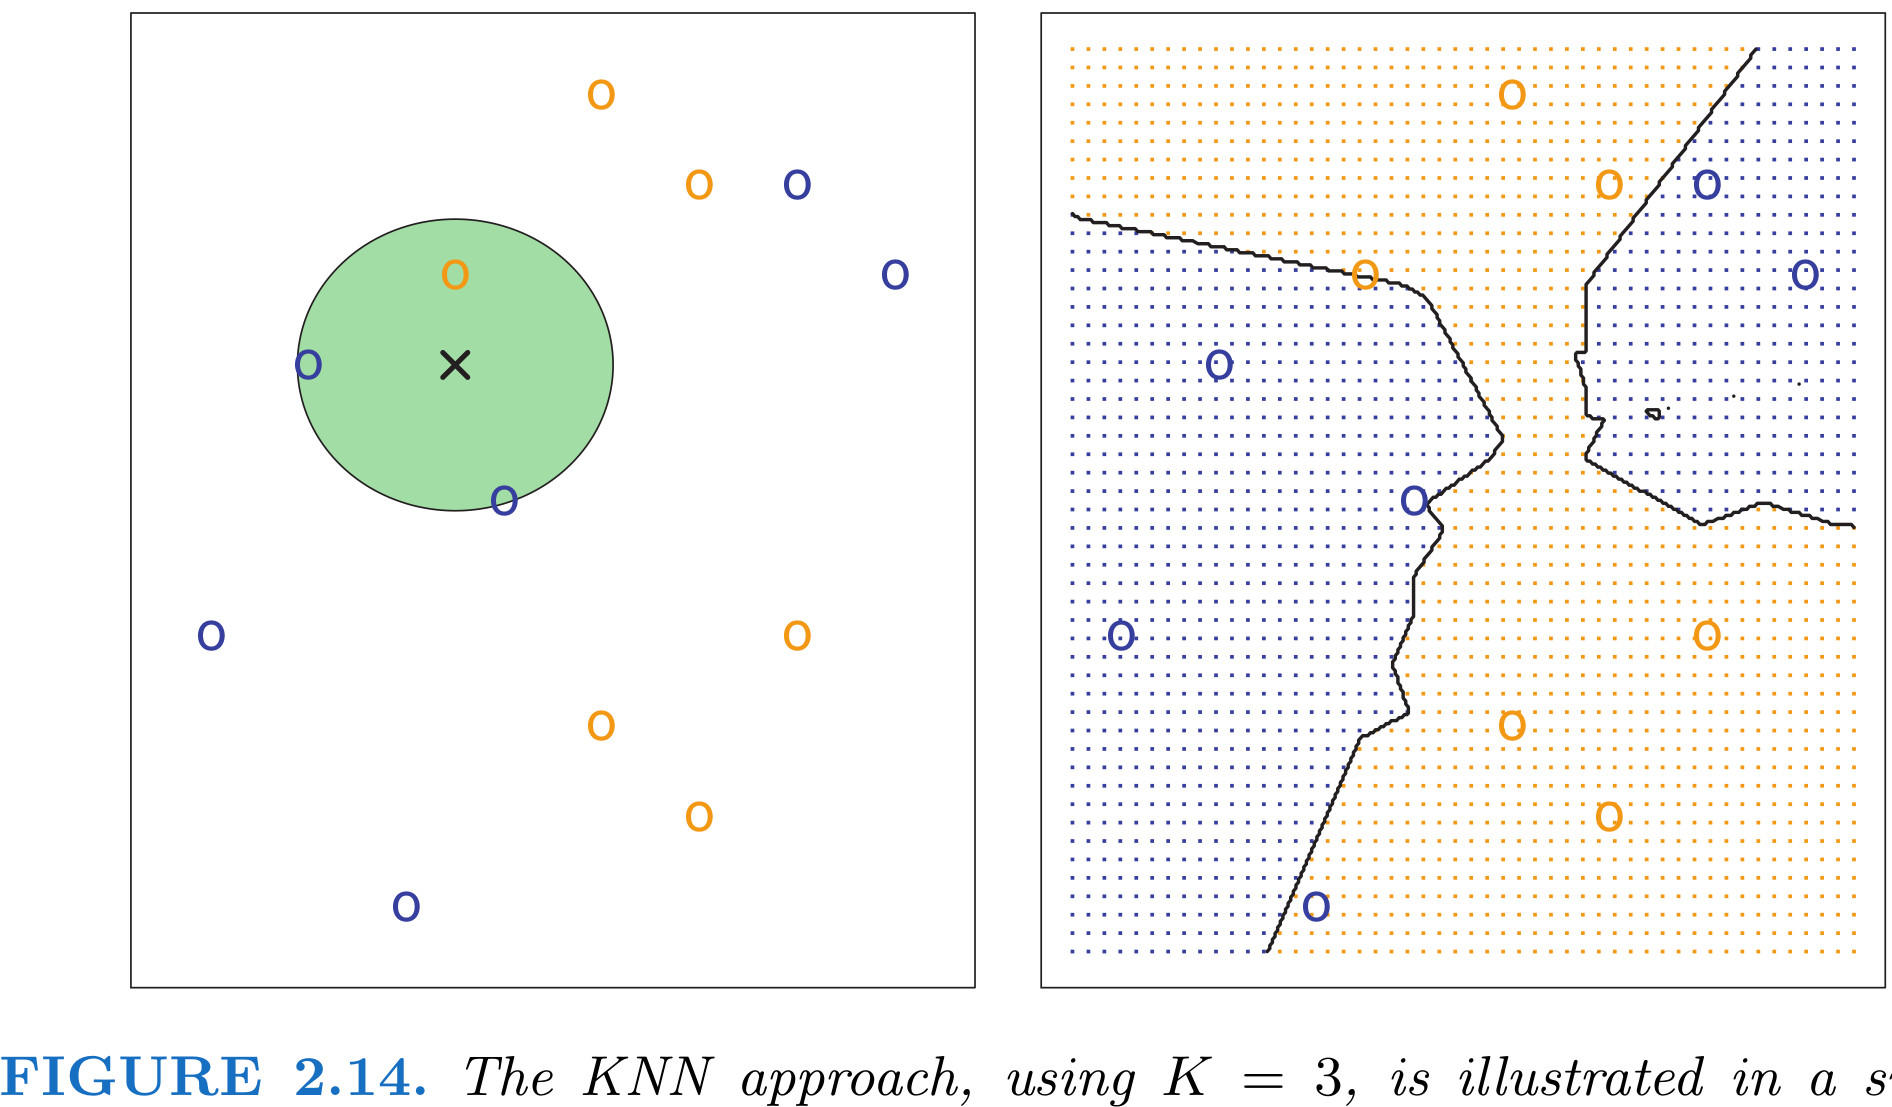
\includegraphics[width=0.78\textwidth]{pics/KNN-classification}
\end{frame}

\section{Discriminative}


\begin{frame}{Discriminative classifier}
	Directly model $p(Y = k | X)$ as a function of $X$.
	
	
	$$p(Y = k | X) = f(X)$$
	
\end{frame}
\begin{frame}{Logistic regression}
	
	$$p(Y = 1 | X) = logit^{-1}(\beta_0 + \beta_1 X) = \frac{e^{\beta_0 + \beta_1 X}}{1 + e^{\beta_0 + \beta_1 X}}$$
	
	\begin{figure}
		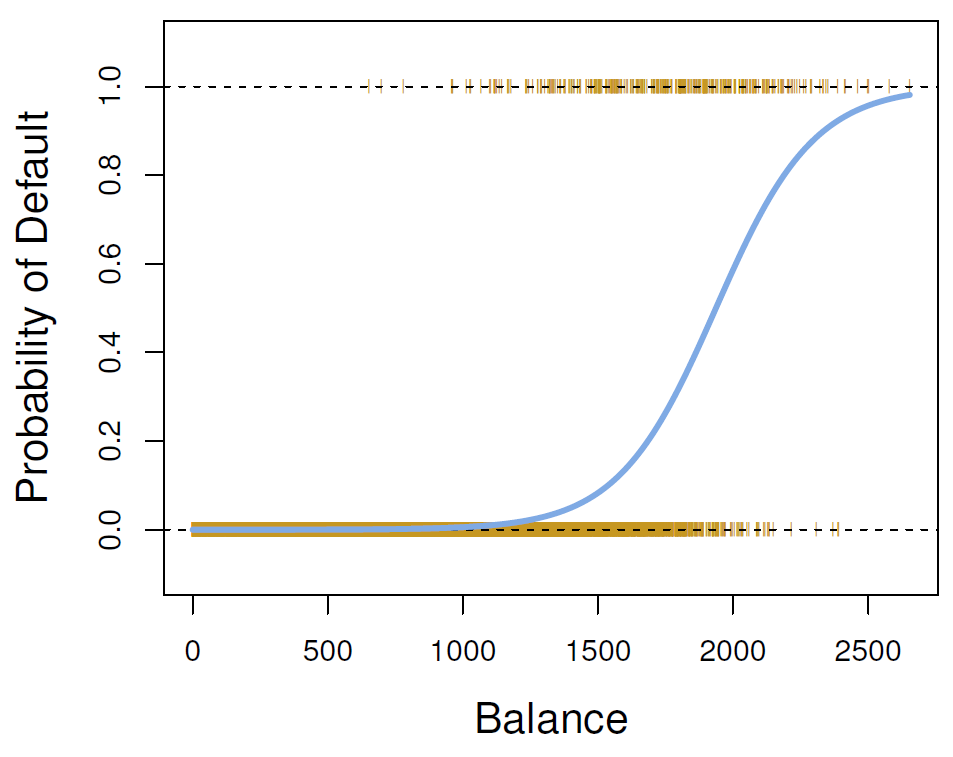
\includegraphics[width=0.4\textwidth]{pics/logistic.png}
	\end{figure}
	
	
 	\,\hfill$\beta_0 = -10.65$, $\beta_1 = 0.0055$
	
\end{frame}

\begin{frame}{Logistic regression}
	Turning this function around:
	
	$$log\left(\frac{p(Y = 1 | X)}{1-p(Y = 1 | X)}\right) = \beta_0 + \beta_1 X$$
	
	Get comfortable with odds, log-odds, the logit, and the inverse logit!
	
\end{frame}

\begin{frame}{Logistic regression}
	$$log\left(\frac{p(Y = 1 | X)}{1-p(Y = 1 | X)}\right) = \beta_0 + \beta_1 X$$
	
	If  $\beta_0 = 0; \beta_1 = 2$:	Interpretation for log-odds? \\
	
	When $X$ increases by 1, the log-odds of $Y = 1$ increase by 2. \\
	
\end{frame}

\begin{frame}{Logistic regression}
	$$\frac{p(Y = 1 | X)}{1-p(Y = 1 | X)} = e^{\beta_0 + \beta_1 X}$$
	
	If  $\beta_0 = 0; \beta_1 = 2$:	Interpretation in odds?\\
	
	When $X$ increases by 1, the odds of $Y = 1$ multiply by $e^2 = 7.39$ \\
	
\end{frame}

\begin{frame}{Logistic regression}
	$$p(Y = 1 | X) = \frac{e^{\beta_0 + \beta_1 X}}{1 + e^{\beta_0 + \beta_1 X}}$$
	
	If  $\beta_0 = 0; \beta_1 = 2$:	Interpretation in probabilities?\\
	
	\begin{itemize}
		\item When $X$ increases from 0 to 1, $Pr(Y = 1)$ increases from  $logit^{-1}(0 + 2 \cdot 0) = 0.5$ to $logit^{-1}(0 + 2 \cdot 1) \approx 0.88$\\
		\item When $X$ increases from 1 to 2, $Pr(Y = 1)$ increases from  $logit^{-1}(0 + 2 \cdot 1) \approx 0.88$ to $logit^{-1}(0 + 2 \cdot 2) \approx 0.98$\\
	\end{itemize}	
	
	Tip: use predicted probabilities (\texttt{predict(model, type = "response")} function in R)
\end{frame}

\section{Generative}

\begin{frame}{Generative classifier}
	Use Bayes' rule to get to $p(Y = k | X)$.
	
	
	$$p(Y = k | X) = \frac{\pi_k \cdot p(X | Y = k)}{\sum_{k = 1}^K \pi_k \cdot p(X | Y = k)}$$

\end{frame}

\begin{frame}{Linear discriminant analysis}
	\begin{itemize}
		\item $\pi_k$ is the proportion of observations in class $k$
		\item $p(X | Y = x)$ is a normal distribution with mean $\mu_k$ and common variance $\sigma^2$
	\end{itemize}
	
	\begin{figure}
		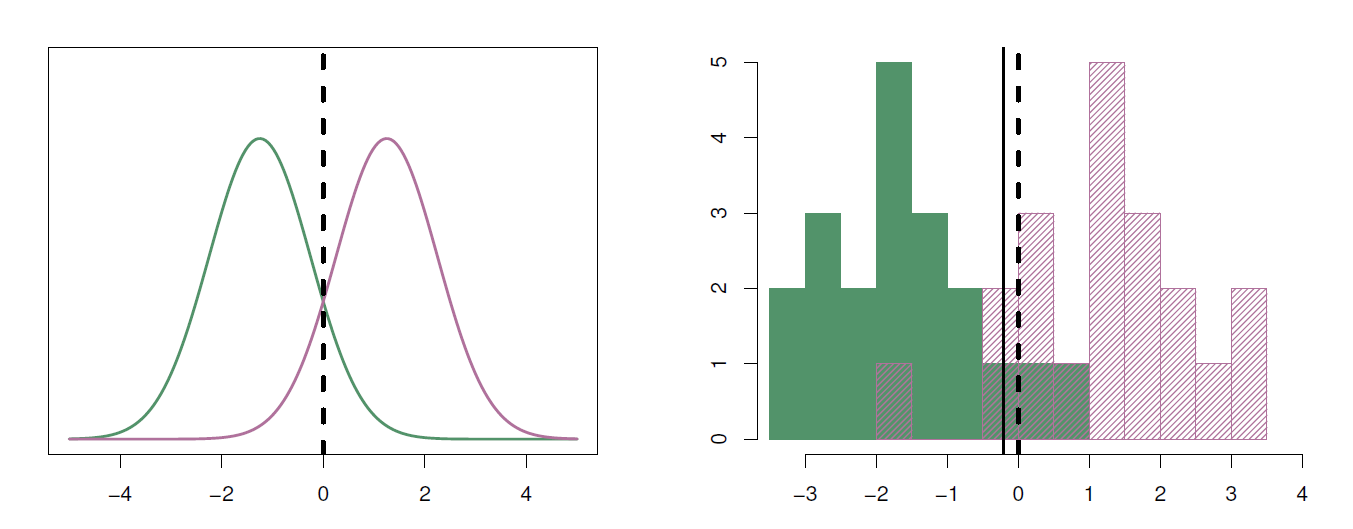
\includegraphics[width=0.78\textwidth]{pics/lda.png}
	\end{figure}
\end{frame}

\begin{frame}{Linear discriminant analysis}
	Advantages over logistic regression:
	\begin{itemize}
		\item Easy to extend to K > 2 classes
		\item Really easy to estimate (analytic solution for $\mu_k$ and $\sigma^2$). You can program it yourself!
		\item You can generate new $X$ from the model (generative model).
	\end{itemize}

	Disadvantages:
	\begin{itemize}
		\item Assumption that $X$ is normally distributed within each class $k$ (categorical predictors???)
		\item Assumption that the variance of each normal distribution is the same!
	\end{itemize}
\end{frame}

\begin{frame}{Linear discriminant analysis}
	Discriminative classifiers
	\begin{itemize}
		\item Directly model $p(Y = k | X)$, for example using the logit link function.
	\end{itemize}
	\vfill
	Generative classifiers
	\begin{itemize}
		\item Estimate $p(X | Y = k)$ and $\pi_k$
		\item Use Bayes' rule to turn this into $p(Y = k | X)$:
		$$p(Y = k | X) = \frac{\pi_k \cdot p(X | Y = k)}{\sum_{k = 1}^K \pi_k \cdot p(X | Y = k)}$$
	\end{itemize}
\end{frame}

\section{Break}
\begin{frame}
	Break
\end{frame}


\section{Trees!}
\subsection{}
\begin{frame}
	Trees!
\end{frame}

\begin{frame}
	Using decision trees for prediction
\end{frame}


\begin{frame}{Decision tree: should I buy a car?}
	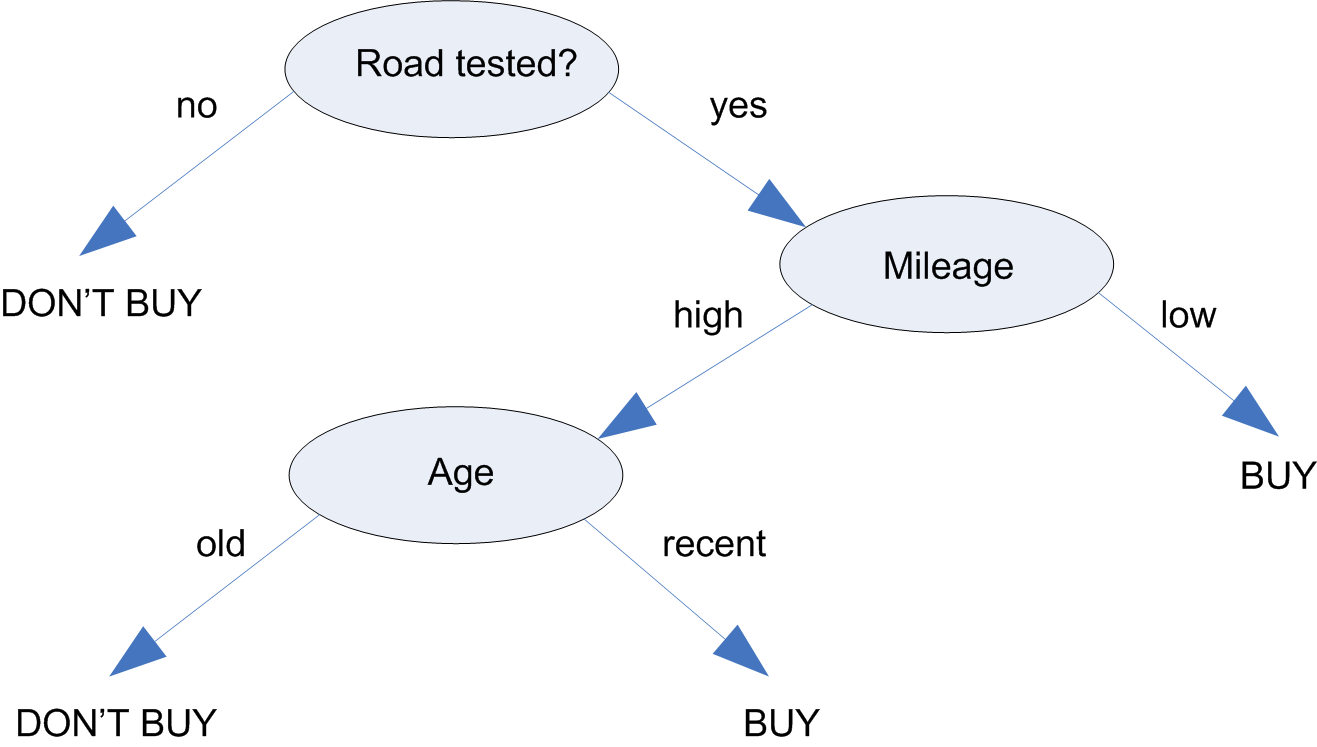
\includegraphics[width=0.78\textwidth]{pics/dectree}
\end{frame}

\begin{frame}{Prediction tree: wood you survive the \emph{Titanic}?}
	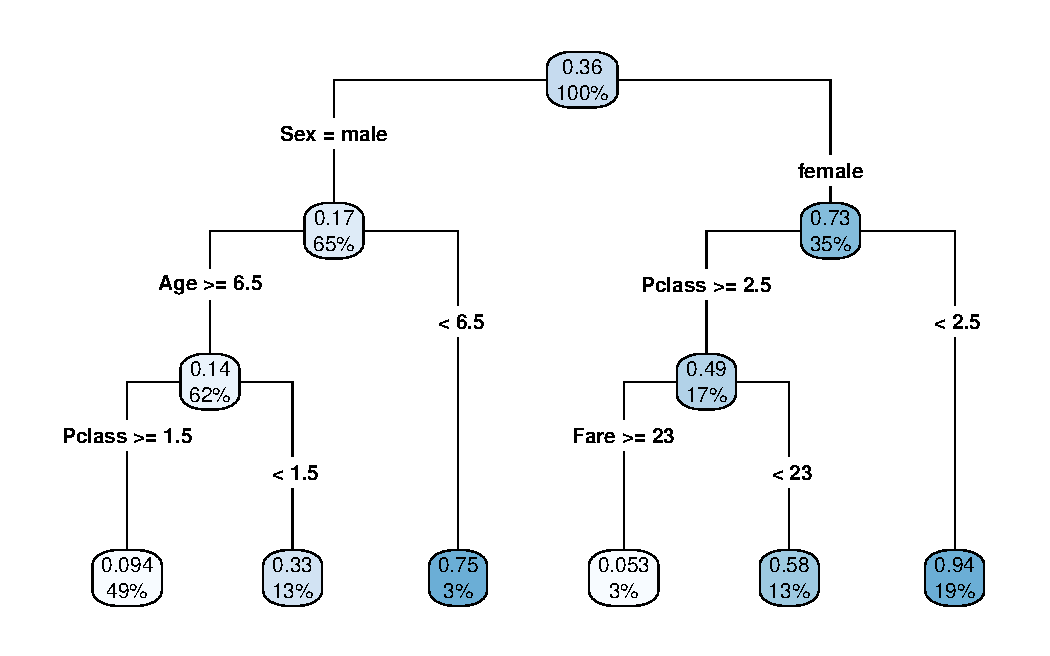
\includegraphics[width=0.78\textwidth]{pics/Titanic_tree}
\end{frame}

\begin{frame}
	Growing decision trees from data 
\end{frame}

\begin{frame}{Recursive partitioning}
	\begin{enumerate}
		\item Find the split that makes observations as similar as possible on the outcome within that split;
		\item Within each resulting group, do (1).
	\end{enumerate}
\end{frame}

\begin{frame}{Recursive partitioning}
	\begin{enumerate}
		\item Find the split that makes observations as similar as possible on the outcome within that split;
		\item Within each resulting group, do (1).
	\end{enumerate}
	
	\bigskip
	\begin{itemize}
		\item Criteria for ``as similar as possible'': Purity, Reduction in MSE, ...
		\item Early stopping: add after (2):
		\begin{itemize}
			\item ``unless there are fewer than $n_{\text{min}}$ observations in the group'' (typically 10);
			\item ``unless the total complexity of the model becomes more than $cp$'' (typically 0.05);
		\end{itemize}
	\end{itemize}
\end{frame}

\begin{frame}
	Simple example
\end{frame}

\begin{frame}
	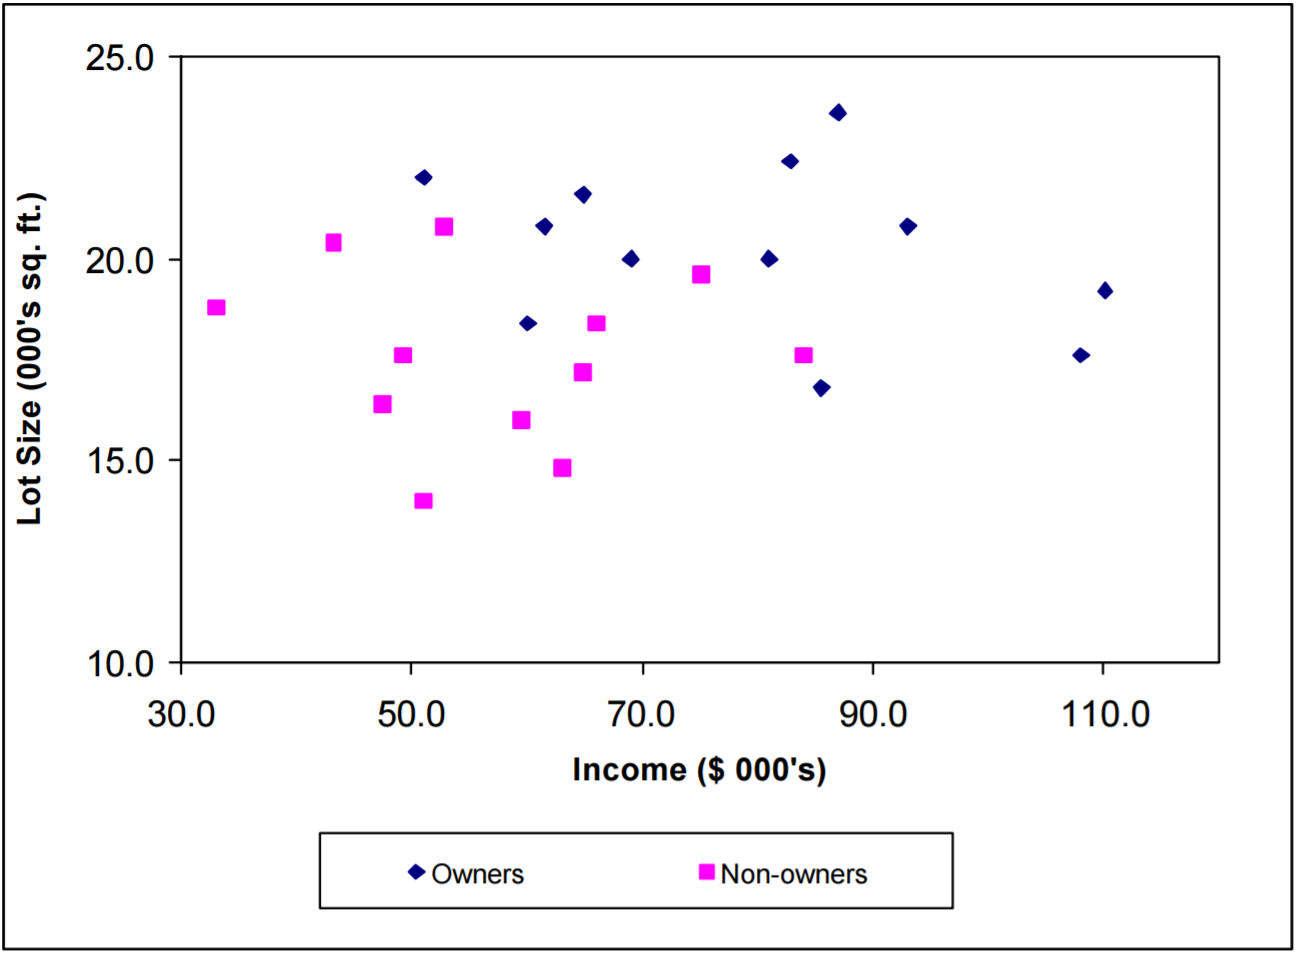
\includegraphics[height=\textheight]{pics/tree1.png}
\end{frame}
\begin{frame}
	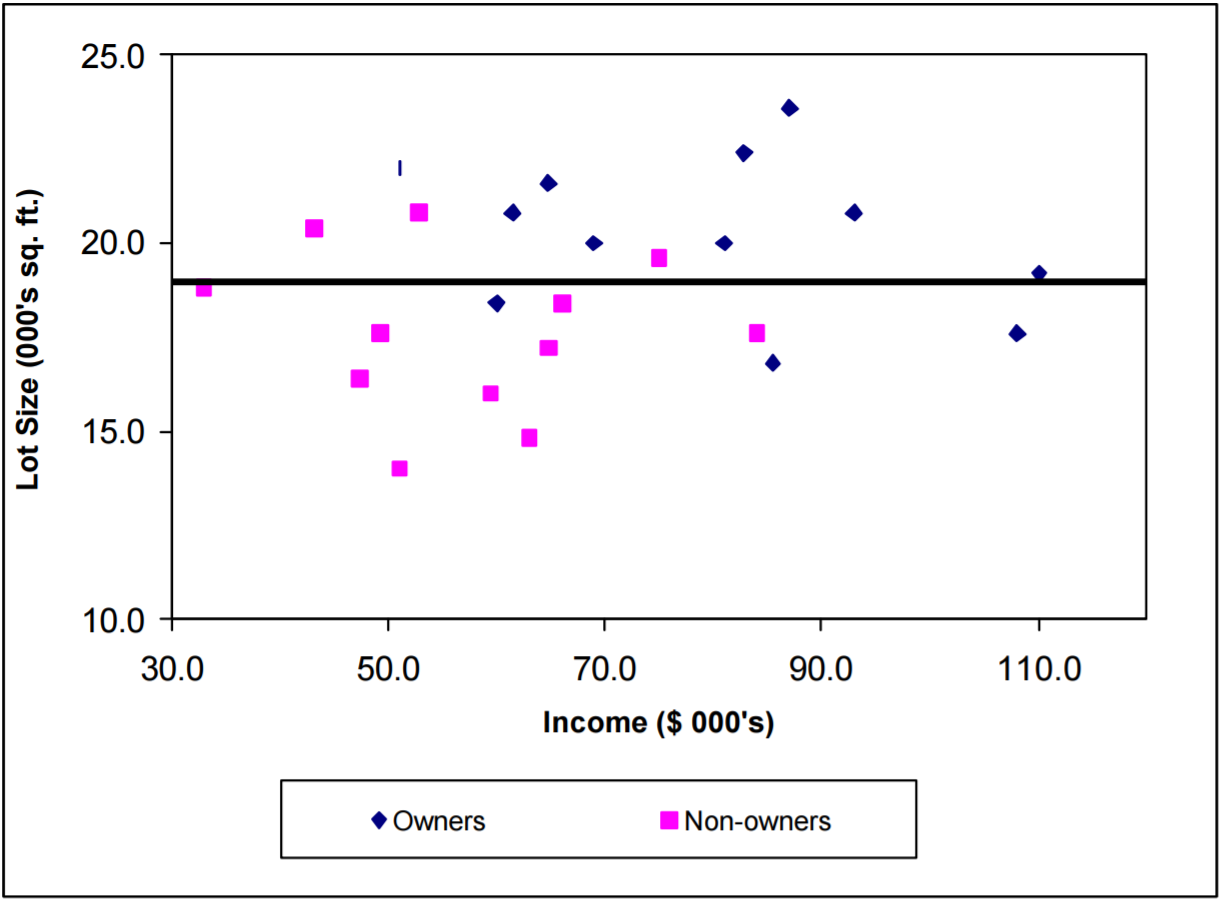
\includegraphics[height=\textheight]{pics/tree2.png}
\end{frame}

\begin{frame}
	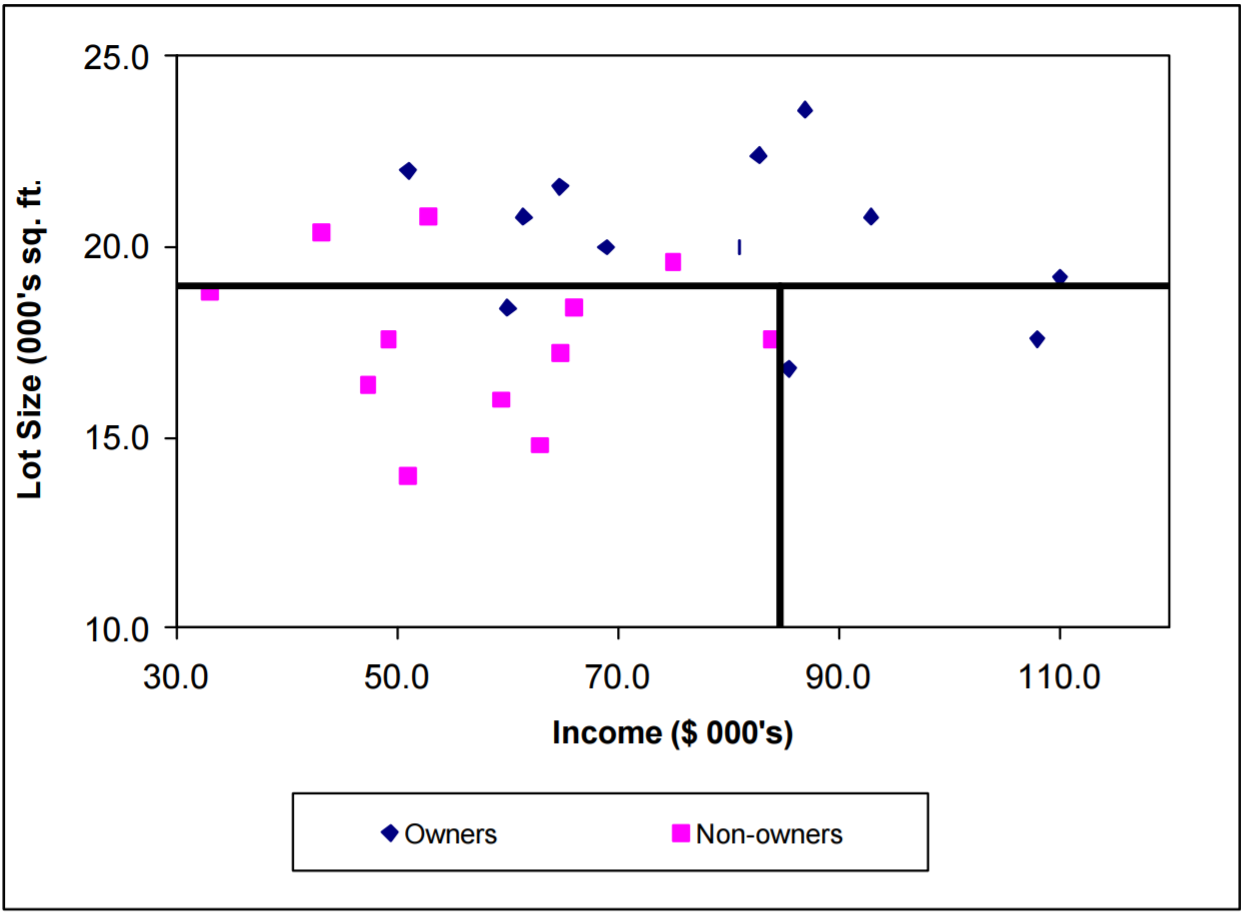
\includegraphics[height=\textheight]{pics/tree3.png}
\end{frame}
\begin{frame}
	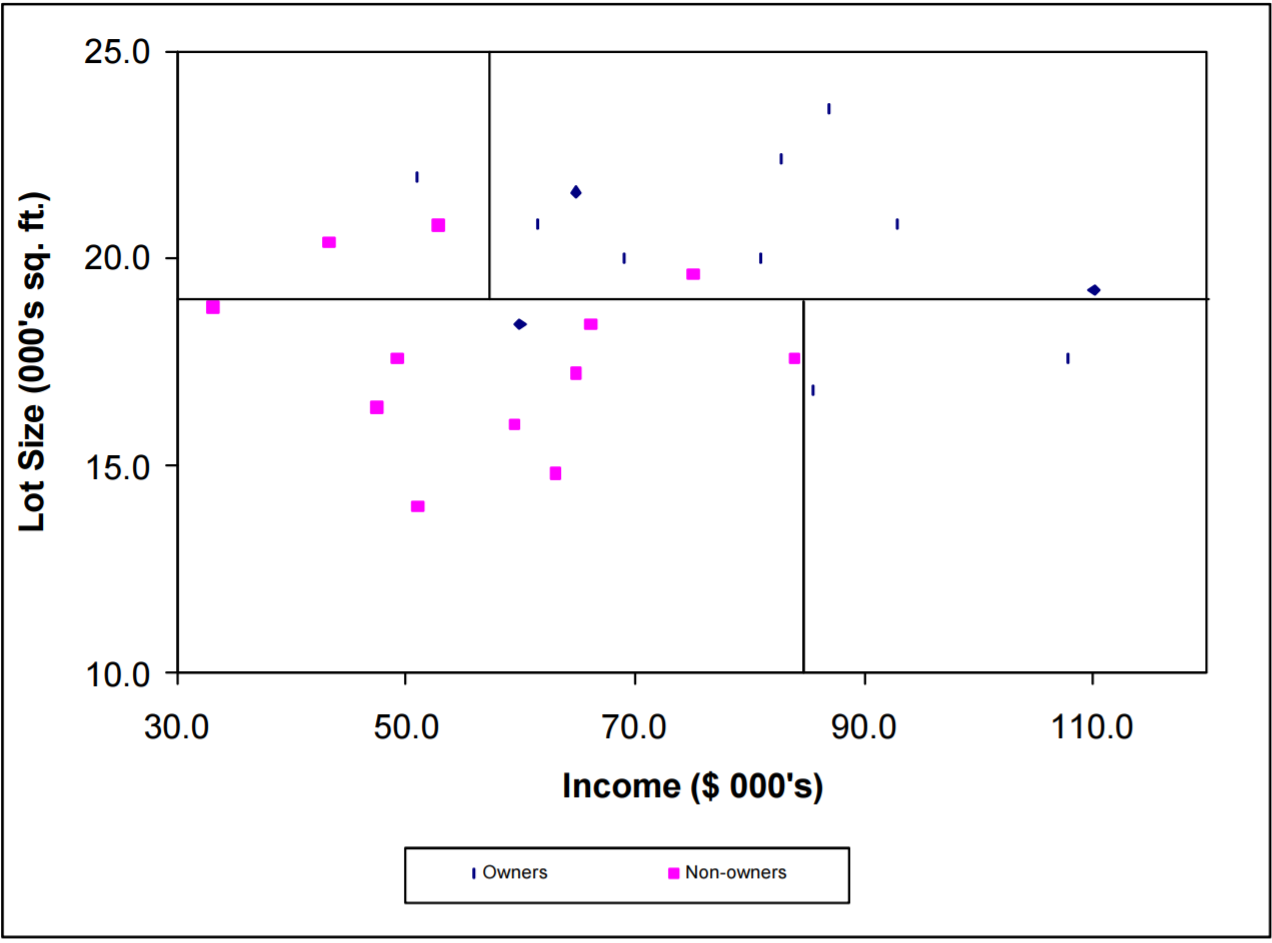
\includegraphics[height=\textheight]{pics/tree4.png}
\end{frame}
\begin{frame}
	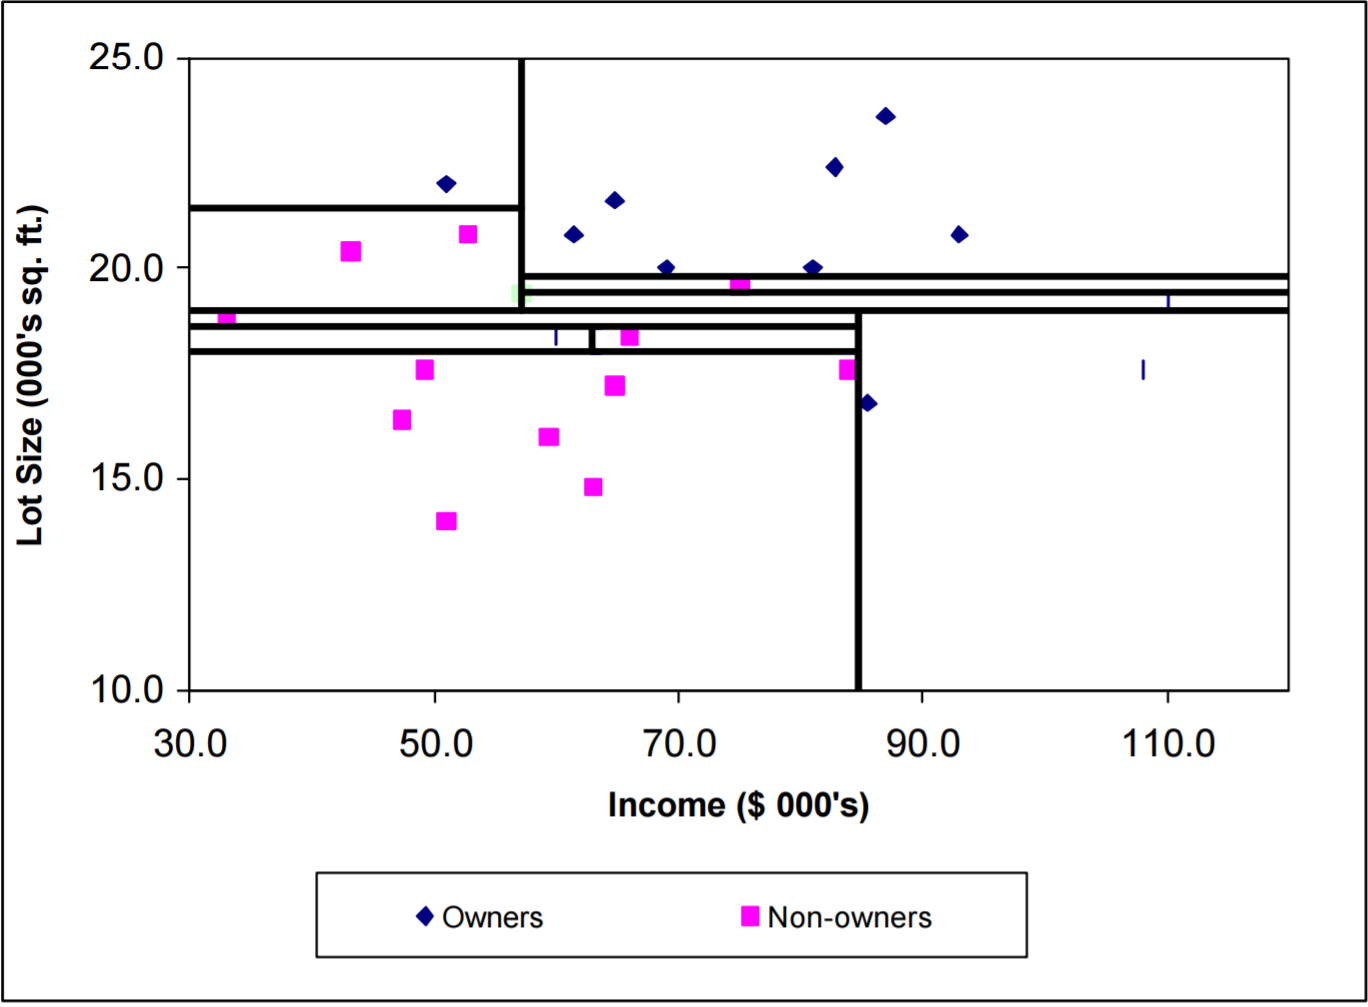
\includegraphics[height=\textheight]{pics/tree5.png}
\end{frame}
\begin{frame}
	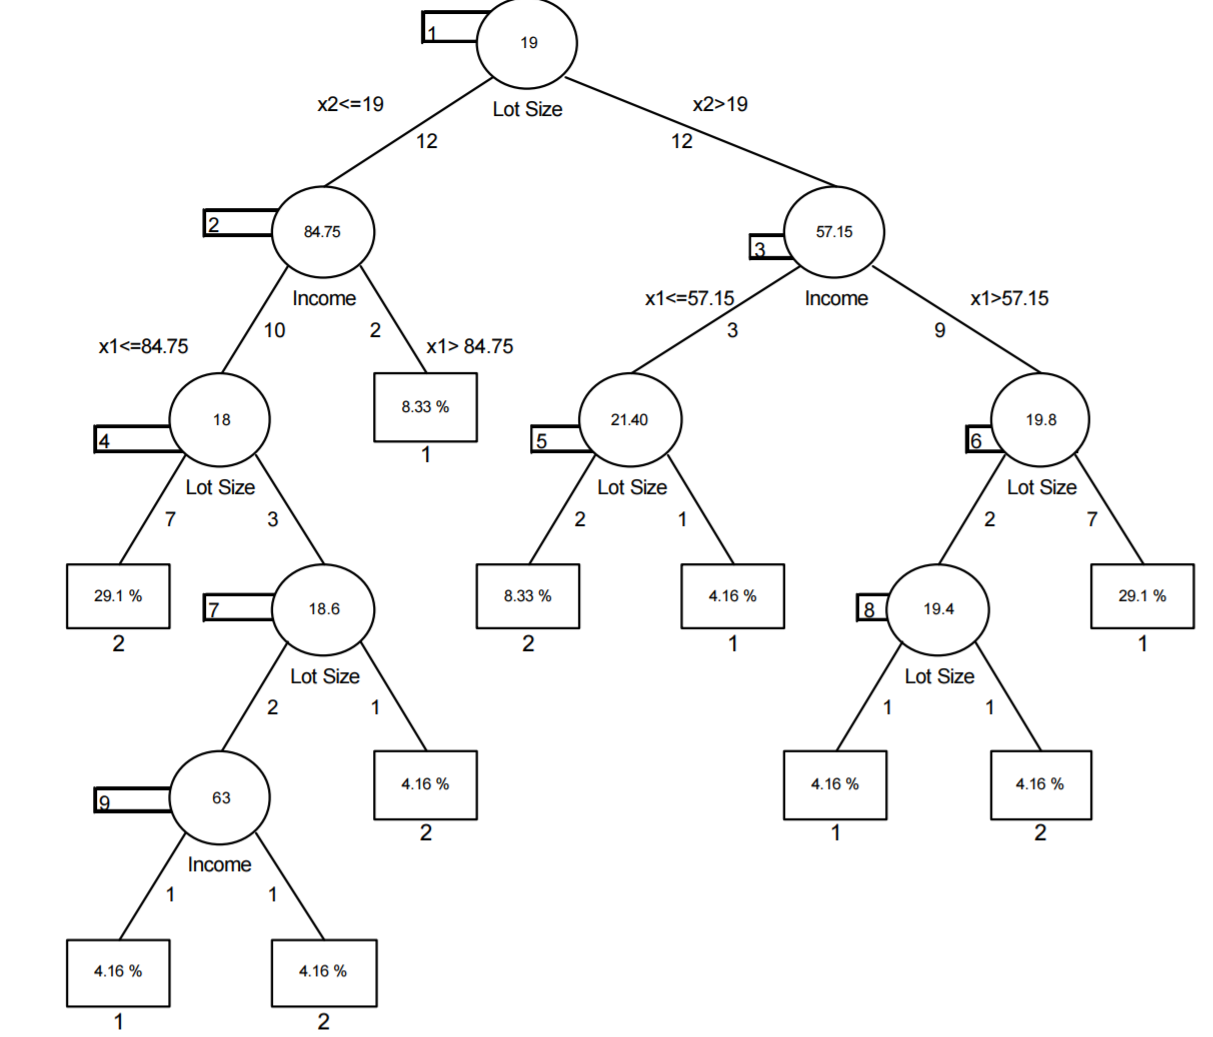
\includegraphics[height=\textheight]{pics/tree_final.png}
\end{frame}
\begin{frame}
	More interesting example
\end{frame}


\begin{frame}
	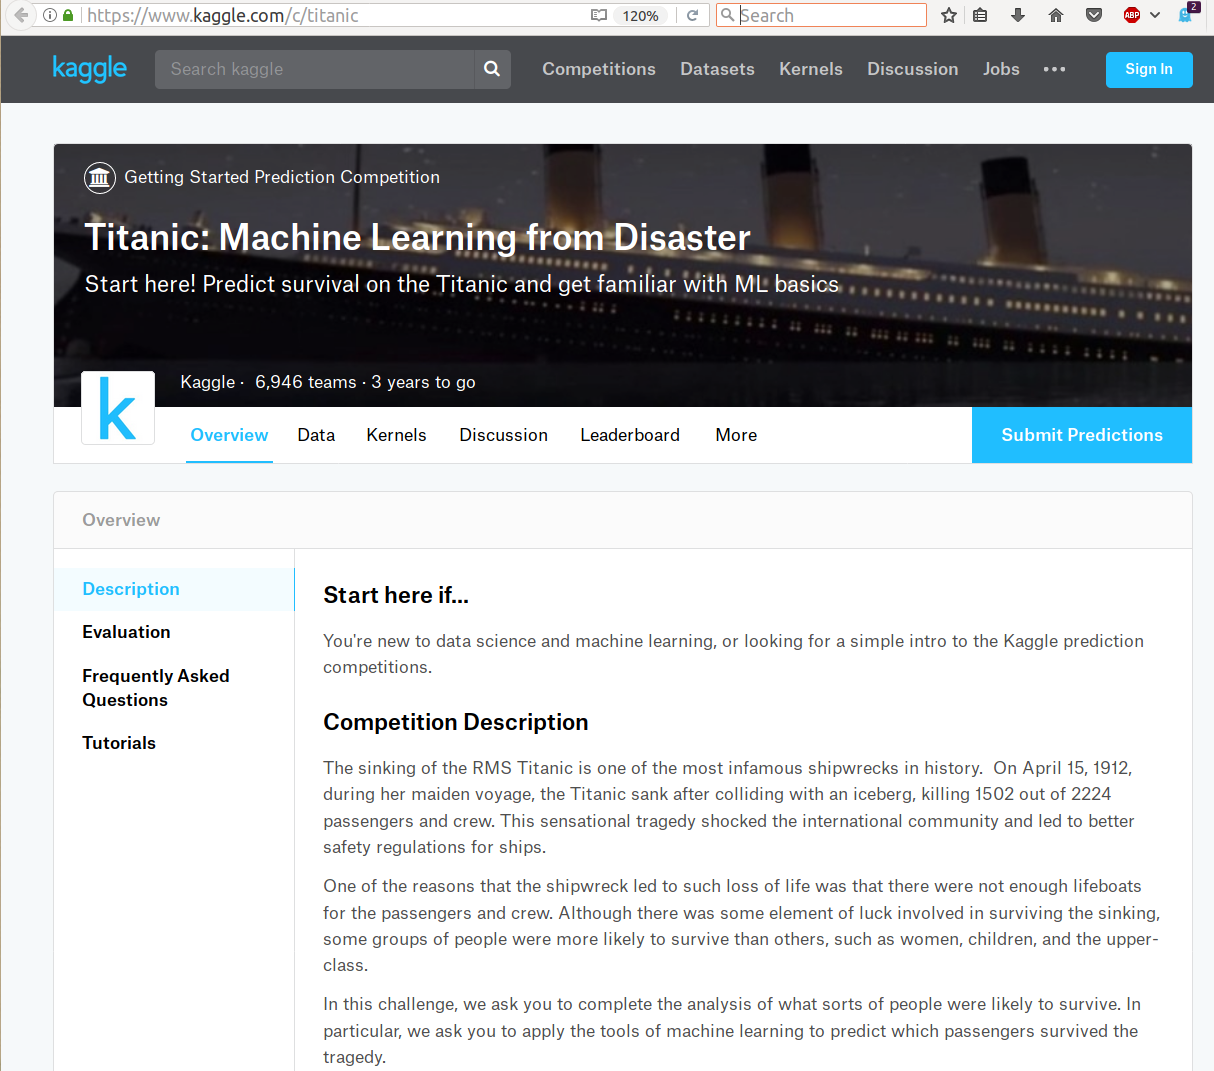
\includegraphics[height=\textheight]{pics/kaggle_scr.png}
\end{frame}
\begin{frame}
	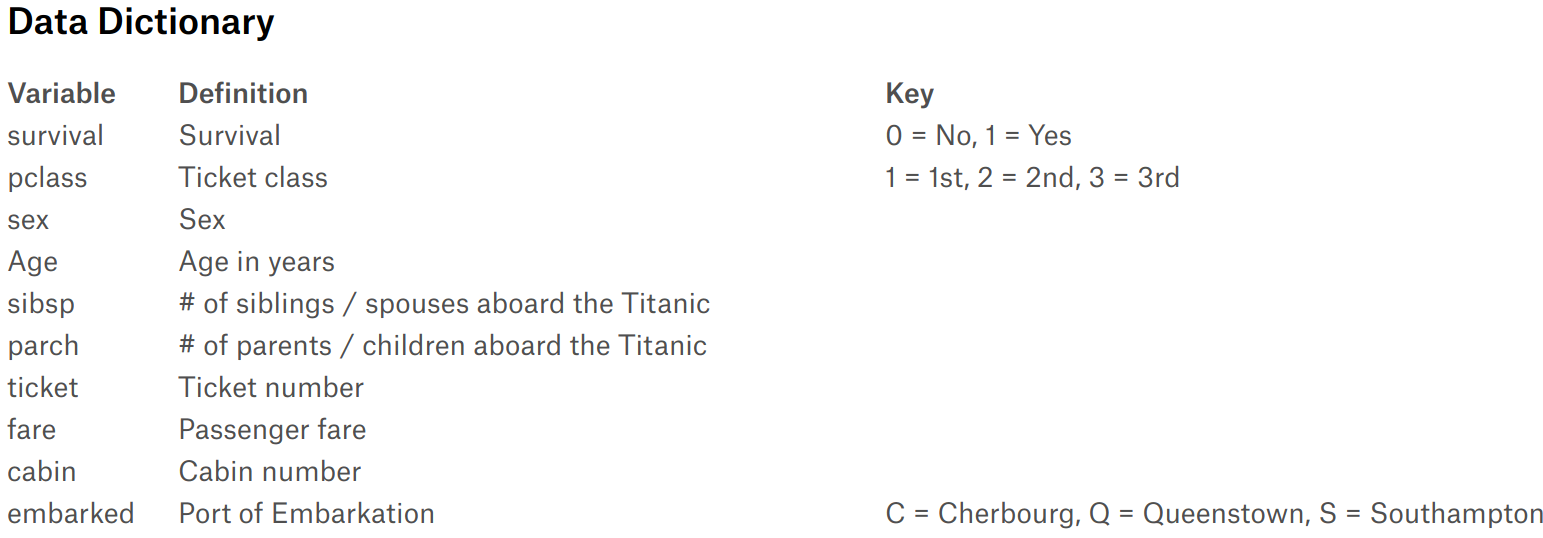
\includegraphics[width=\textwidth]{pics/scr_dict.png}
\end{frame}

\begin{frame}[fragile]{Getting the Titanic data from Kaggle}
	\begin{scriptsize}
		\begin{verbatim}
library(tidyverse)

# Import the Titanic data from Kaggle
train_url <- 
"http://s3.amazonaws.com/assets.datacamp.com/course/Kaggle/train.csv"
titanic_df <- read_csv(train_url)

# Make sure the results are reproducible
set.seed(1027)

# Split the data into 70% train and 30% validation data
N <- nrow(titanic_df)
idx_train <- sample(1:N, size = round(N * 0.7))
train_df <- titanic_df[idx_train, ] # Training data
val_df <- titanic_df[-idx_train, ] # Validation data
\end{verbatim}
	\end{scriptsize}
\end{frame}

\begin{frame}
	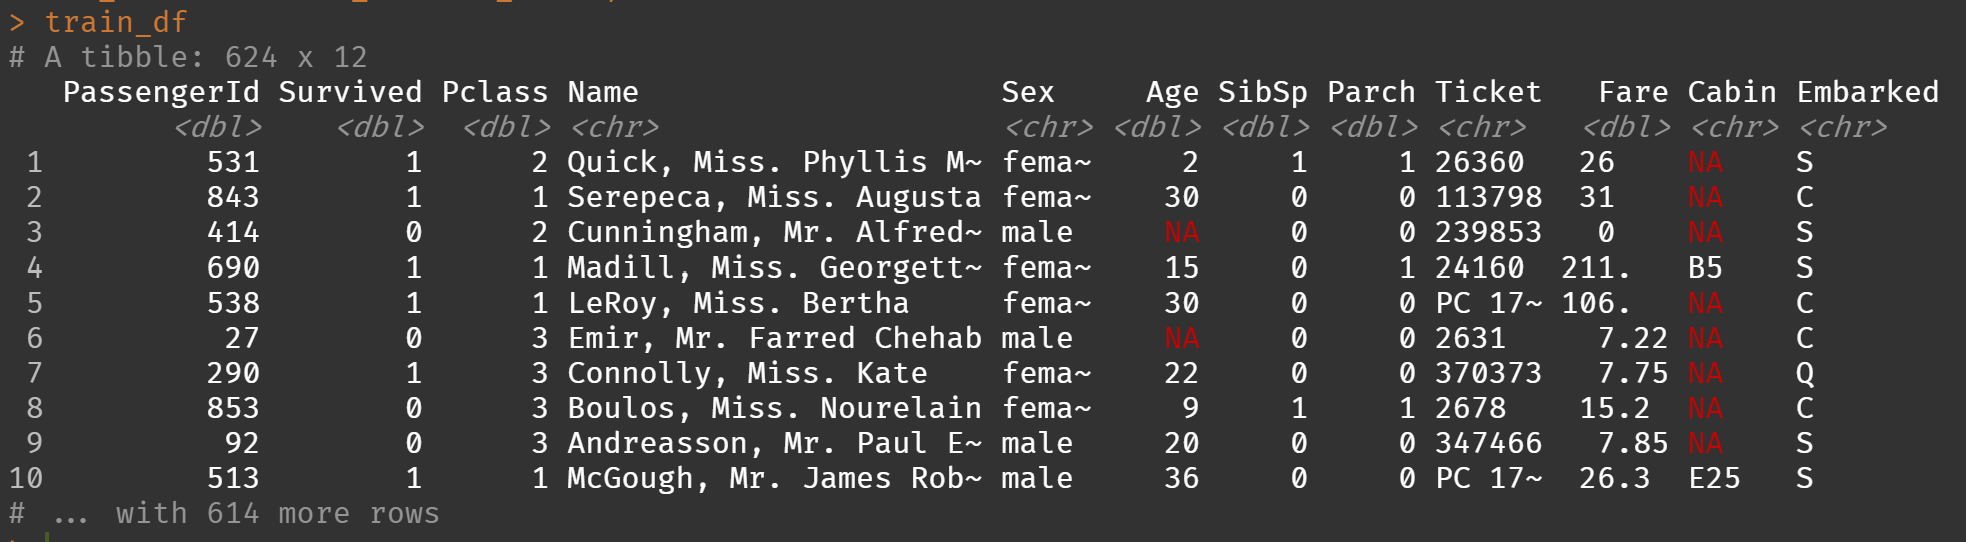
\includegraphics[width=\textwidth]{pics/titanic_scr}
\end{frame}


\begin{frame}[fragile]{Fitting a classification tree in R}
	
	\begin{scriptsize}
		\begin{verbatim}
library(rpart)
library(rpart.plot)

titanic_tree <- 
  rpart(
    Survived ~ Pclass + Sex + Age + SibSp + Parch + Fare + Embarked, 
    data = train_df, 
    control = list(cp = 0.02)
  )
  
rpart.plot(titanic_tree)

\end{verbatim}
		
	\end{scriptsize}
\end{frame}

\begin{frame}
	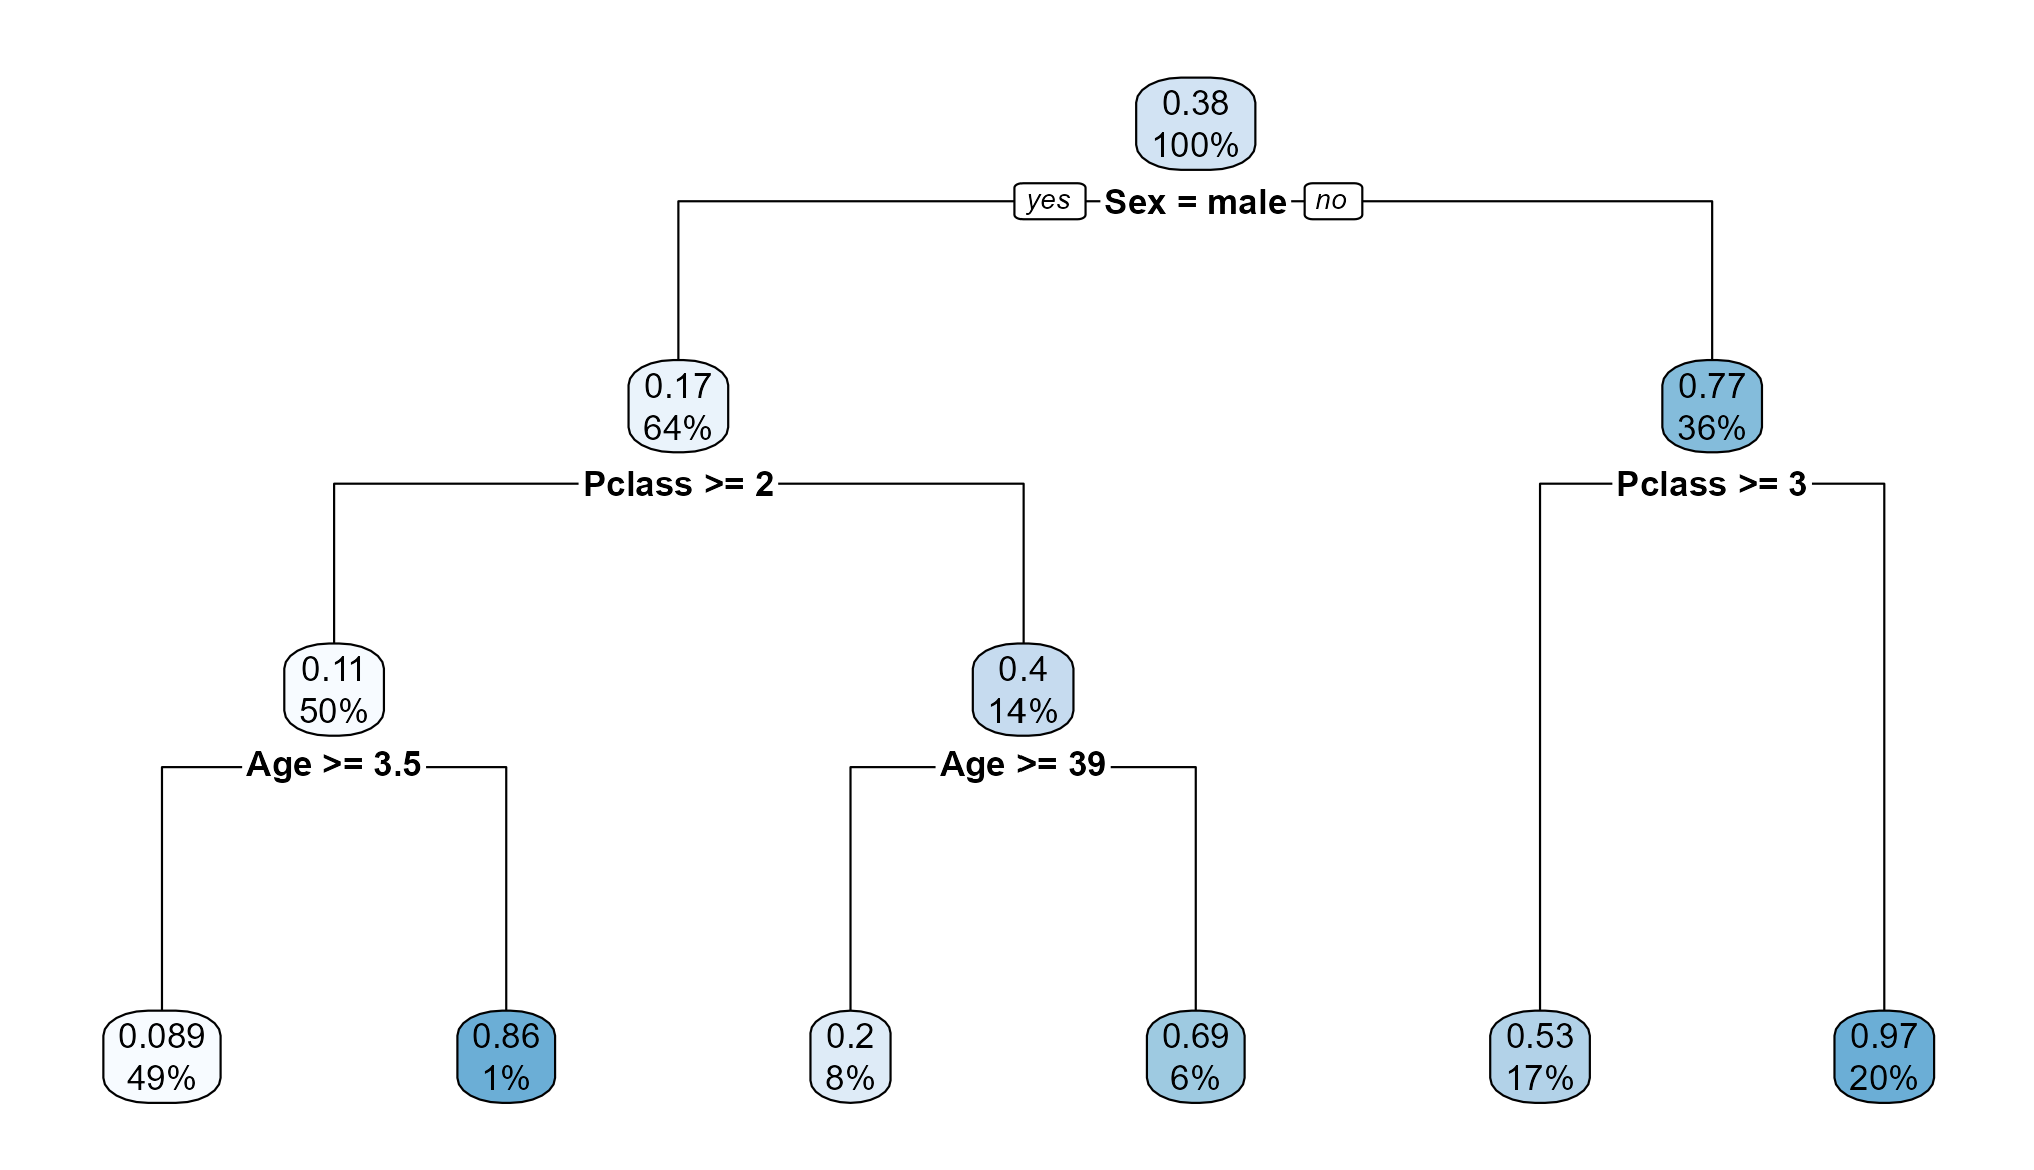
\includegraphics[width=\textwidth]{pics/rpart_plot}
\end{frame}

\section{Evaluating classifiers}
\begin{frame}{Evaluating classifiers}
	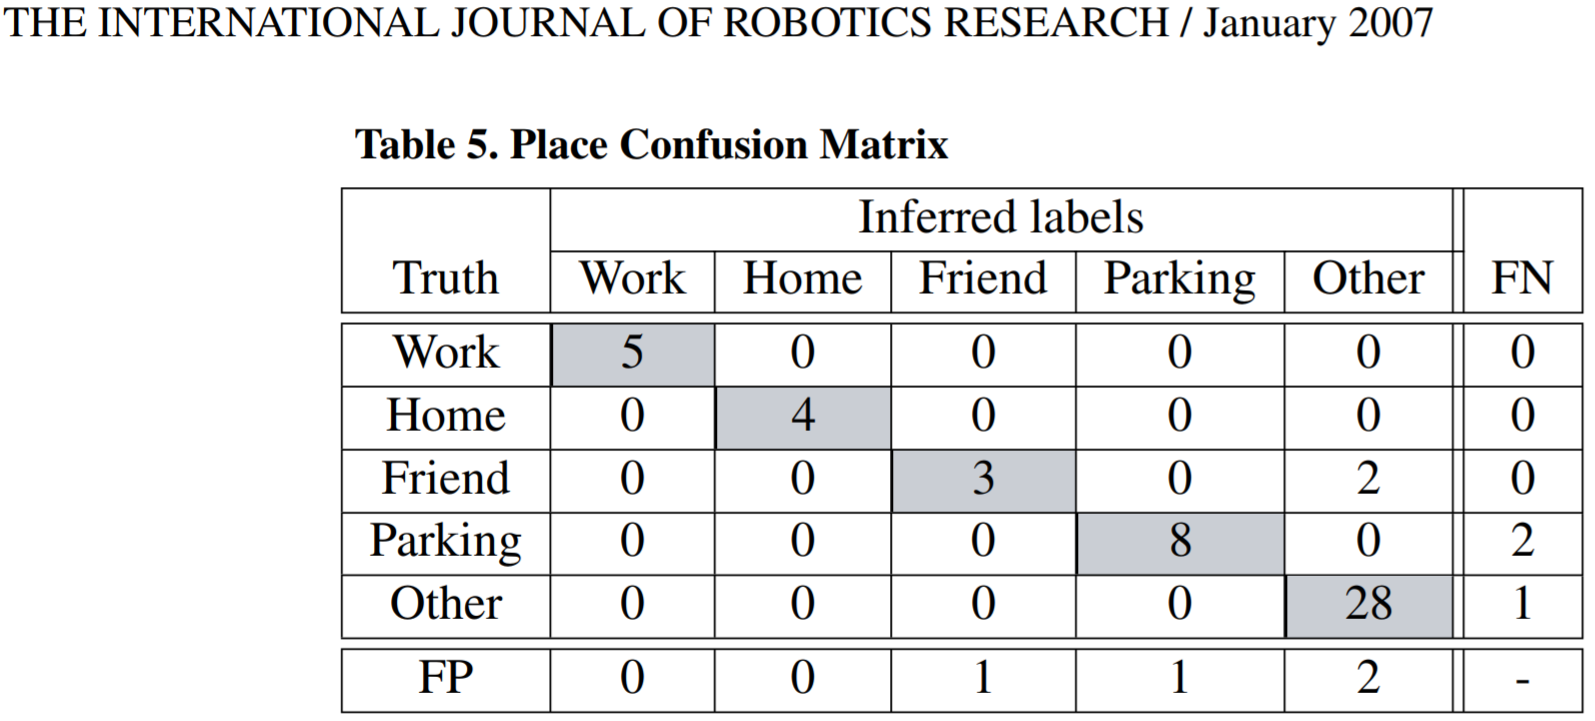
\includegraphics[width=\textwidth]{pics/confusion-place.png}
\end{frame}

\begin{frame}
More on this next week.\\
Wednesday: Q\&A session for practical.
\vfill
	
  \begin{center}
  \emph{Have a nice day!}
  \end{center}

\end{frame}
\end{document}

